\documentclass[a4paper]{article}
\usepackage[margin=1in]{geometry}
\usepackage{graphicx}
\usepackage{subfigure}
\usepackage{ctex}
\usepackage{float}
\usepackage{emoji}

\title{\heiti\zihao{2} TSCTF-J WriteUp}
\author{\songti\zihao{4} Cyber\_Rubbish}
\date{2023.09.24}        
\begin{document}
    \maketitle
\tableofcontents
\section{misc\_尊嘟假嘟}

打开题目附件,是一段音频,按照内容记下,得到如下内容:
并由内容仅为“尊嘟”、“假嘟”,推测为Morse Code, 尊嘟为“-”,假嘟为“.”,解码得到flag。
\begin{figure}[H]
    \centering
    \subfigur{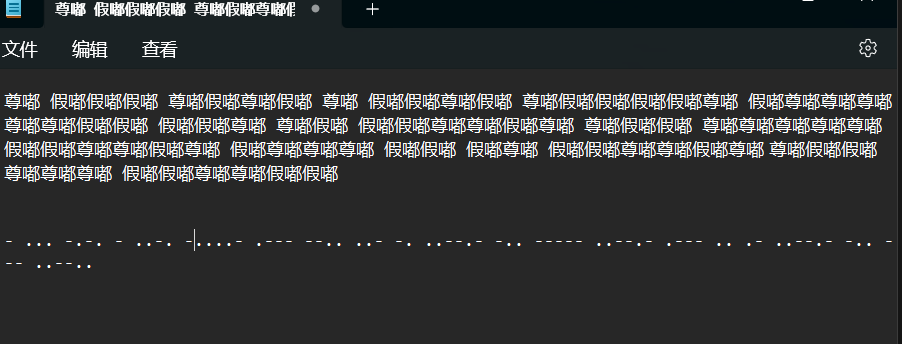
\includegraphics[width=0.8\textwidth]{img/zundujiadu_01.png}}
    \subfigur{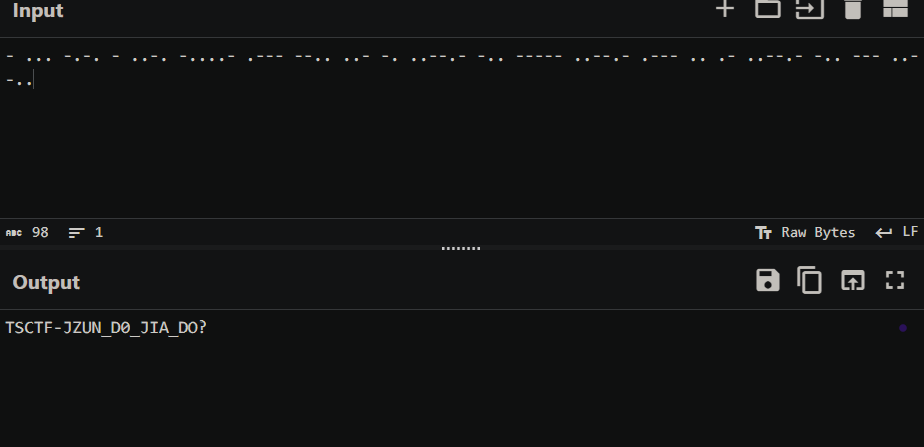
\includegraphics[width=0.8\textwidth]{img/zundujiadu_02.png}}

\end{figure}
\section{misc\_调查问卷}
略\dots
\section{web\_十年之约}
打开题目环境,按照表格,回答够50次正确,即可得到flag。
\section{ab\_abstract\&music}
抽象题,一言难尽,略\dots
\section{总结}
菜鸡本姬.jpg
\end{document}

